\chapter{Lösungsvorschläge}
\label{cha:Lösungsvorschläge}

\section{Framework}
\label{sec:Framwork}

Gesucht ist ein Framework mit dem alle \textit{Muss-Kriterien} bestmöglich umgesetzt werden können. Des Weiteren sollen alle Tasks im Gantt-Diagramm \ref{img:gantt} fristgerecht erledigt werden können. Um das Projekt im genannten Zeitraum durchführen zu können, beschränken wir uns bei der Suche auf die bekanntesten Frameworklösungen auf dem derzeitigen Markt.

Die zwei bekanntesten Framworks für skalierbare, verteilt arbeitende Software im Zusammenhang mit großen Datenmengen sind \textit{Hadoop} und \textit{Spark}. Sowohl Hadoop als auch Spark werden unter Linux entwickelt und verwenden native Linux Libraries. Daher begrenzt sich unsere Auswahl des zu verwendenden Betriebssystems auf Linux Distributionen. Dies erleichtert zum einen das Einrichten und zum anderen die Wartung des Frameworks.

\subsection{Hadoop}
\label{subsec:Hadoop}

Hadoop ist ein Java-Framwork der Apache Software Foundation zum verteilten Speichern von Daten und zu deren parallelen Verarbeitung. Hadoop wird dabei in einem horizontal skalierbaren Cluster betrieben, das auf einfachstem Weg wie gewünscht skaliert werden kann. Große Unternehmen wie Yahoo betreiben so Cluster mit über 4000 Knoten\footnote{Referenzzahlen für Unternehmen, die Hadoop einsetzen: http://wiki.apache.org/hadoop/PoweredBy}. Statt der Anschaffung neuer, schnellerer Hardware (Scale Up) wird beim Betrieb von Hadoop vielmehr die Erweiterung des Clusters (Scale Out) um weitere Knoten empfohlen.

Zu den Basiskomponenten von Hadoop, die bei der Installation mitgeliefert werden gehören:

\begin{itemize}
\item \textbf{Hadoop Distributed File System (HDFS):} Ein über das gesamte Cluster verteiltes Dateisystem zur Speicherung der zu verarbeitenden Daten.
\item \textbf{Map-Reduce:} Ein Programmierframework zur verteilten Verarbeitung von Daten gemäß der zweiphasigen Verarbeitung durch Mapper- und Reducer-Klassen.
\item \textbf{YARN:} Verwaltet die Resourcen eines Clusters dynamisch für verschiedene Jobs. 
\end{itemize} 

Zudem verfügt Hadoop über ein großes Ökosystem, das zahlreiche Technologien enthält, die ergänzend zu den genannten Technologien, installiert werden können.


\begin{figure}[!htb]
	\centering
	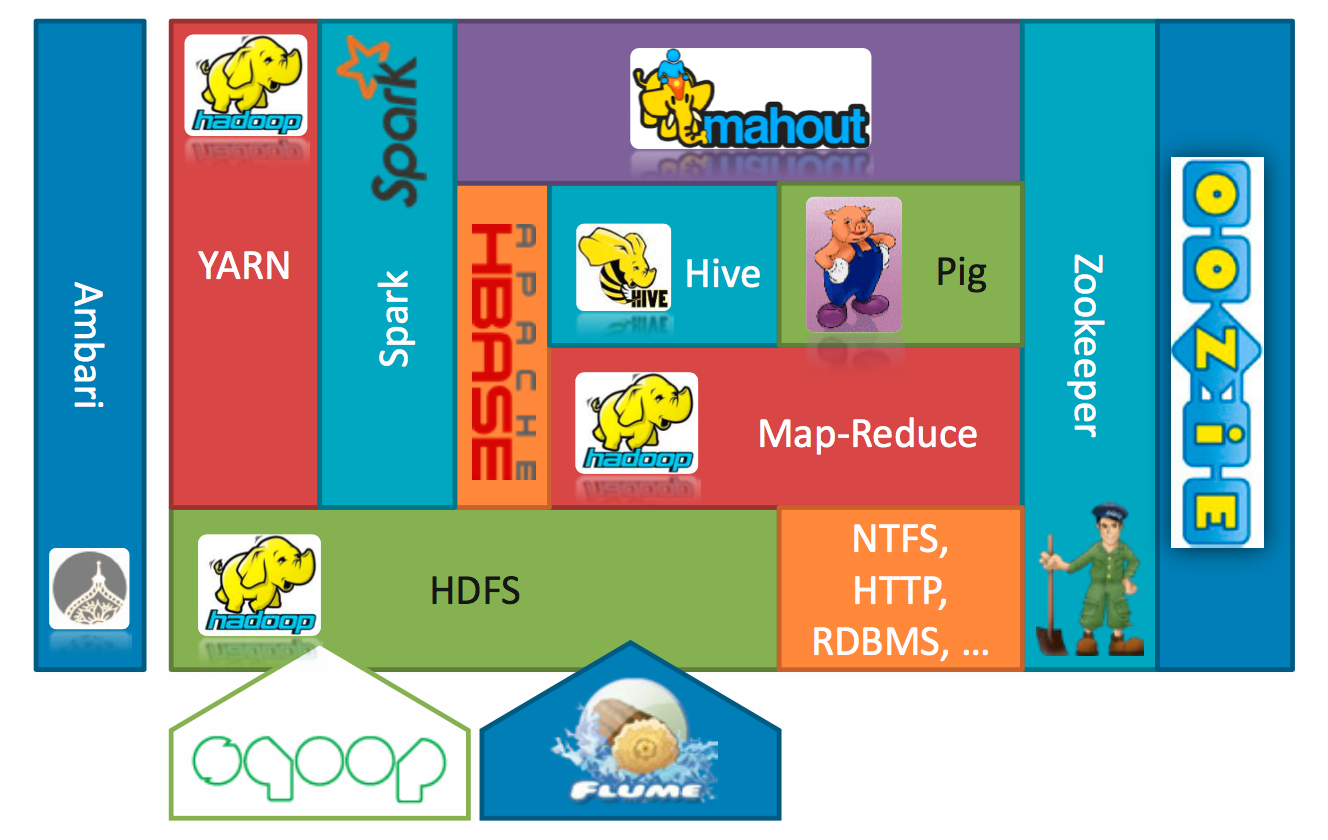
\includegraphics[width=0.8\textwidth]{hadoopecosystem}
	\caption{Hadoop-Ökosystem}
	\label{img:hadoopecosystem}
\end{figure}


\subsection{Spark}
\label{subsec:Spark}

Die Daten-Analyse Plattform Spark für clustergestützte Berechnungen wird hauptsächlich für die schnelle Ausführung von Jobs genutzt. Mit Apache Spark können Daten transformiert, fusioniert sowie mathematischen Analysen unterzogen werden. Spark ist darauf ausgelegt die Daten dynamisch im RAM des Server-Clusters zu halten und dort zu verarbeiten. Die sogenannte In-Memory-Technologie gewährleistet eine extrem schnelle Auswertung riesiger Datenmengen.

Die besondere Stärke ist das beinhaltete maschinelle Lernen (Machine Learning) mit den Zusätzen MLib (Machine Learning Bibliothek) sowie SparkR(Direkte Verwendung von R-Bibliotheken unter Spark). Dadurch lassen sich iterative Schleifen sehr gut verarbeiten was eine wichtige Vorrausetzung für Machine Learning Algorithmen darstellt.

\begin{figure}[!htb]
	\centering
	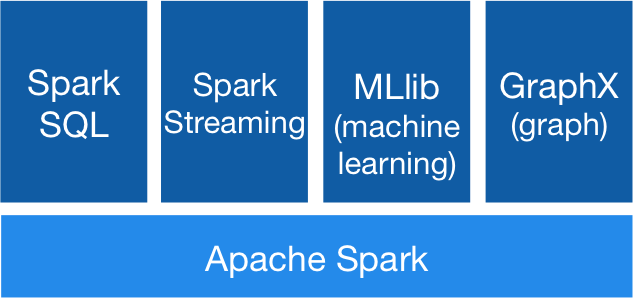
\includegraphics[width=0.5\textwidth]{spark}
	\caption{Apache Spark Framework}
	\label{img:sparkframework}
\end{figure}

\pagebreak

\section{Datenbank}
\label{sec:Datenbank}

\subsection{HBase}
\label{subsec:HBase}

Apache HBase ist eine quelloffene, spaltenorientierte NoSQL-Datenbank, die sich in ihrer Architektur und ihrem Aufbau an Google's \textit{BigTable} orientiert. Eine Besonderheit von HBase ist, dass ein Datensatz beliebig viele Spalten haben kann, auch mehr oder weniger als der vorige oder folgende Datensatz. Diese Eigenschaft hilft bei der schnellen persistenten Speicherung von Daten, da diese zuvor nicht normalisiert werden müssen. HBase ist Teil des Hadoop-Ökosystems \ref{img:hadoopecosystem} und kann daher im \textit{verteilten Modus} ausgeführt werden, in dem sie auf Hadoop aufsetzt und das HDFS nutzt, um ihre Daten darin zu speichern. Der Vorteil beim verteilten Speichern von Daten liegt wie auch beim HDFS darin, besonders große Datenmengen unterzubringen und auf Wunsch zu skalieren, indem man weitere Knoten dem Cluster hinzufügt, wenn Performance oder Speicherkapazitäten knapp werden. Bekannte Unternehmen, die HBase verwenden sind: Adobe, Facebook, Netflix, Spotify, Yahoo! uvm.

\subsection{Cassandra}
\label{subsec:Cassandra}

Apache Cassandra ist ebenfalls eine spaltenorientierte NoSQL-Datenbank, die als skalierbares, ausfallsicheres System für den Umgang mit großen Datenmengen in verteilten Systemen (Clustern) konzipiert wurde. Sie entstand ebenfalls nach dem Vorbild von Google's \textit{BigTable}. Cassandra wird häufig zusammen mit dem Framework Spark verwendet und bildet mit zusätzlichen Technologien den SMACK-Stack, bestehend aus \textbf{S}park, \textbf{M}esos, \textbf{A}kka, \textbf{C}assandra und \textbf{K}afka. Daher wird Cassandra eher mit den genannten Technologien verwendet und harmoniert weniger gut mit Hadoop. Bekannte Unternehmen, die Cassandra verwenden sind: Twitter, Digg und Reddit. Auch Facebook nutzte bis 2011 Cassandra, bis diese durch eine Kombination von HBase und HDFS ersetzt wurde. 

\pagebreak

\section{Virtualisierungssoftware}
\label{sec:Virtualisierung}

\subsection{Docker}
\label{subsec:Docker}

Die Open-Source-Technologie Docker ermöglicht es Anwendungen mithilfe von Betriebssystemvirtualisierung in Containern zu isolieren. Durch die Verwendung von Containern können die Applikationen erstellt, ausgeführt, getestet und verteilt werden. 

Durch das Verpacken von Anwendungen in standardisierte Einheiten erfolgt eine Trennung sowie Verwaltung der auf dem Rechner verwendeten Ressourcen. Diese Einheiten enthalten alle Komponenten die eine Software für die Ausführung benötigt wie z.B. Code, Laufzeitmodul, System-Tools und Systembibliotheken. Dadurch ermöglicht Docker eine schnelle, zuverlässige und einheitliche Bereitstellung von Anwendungen - unabhängig von der Umgebung.

Die Isolation der Anwendungen erfolgt bei Docker auf Software Ebene.

\begin{figure}[!htb]
	\centering
	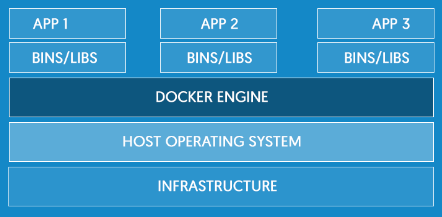
\includegraphics[width=0.5\textwidth]{Docker}
	\caption{Aufbau Docker}
	\label{img:AufbauDocker}
\end{figure}

\subsection{VirtualBox}
\label{subsec:VirtualBox}

Die Virtualisierungssoftware von Oracle ermöglicht die Installation von virtuellen Maschinen auf einem Host System. Dabei greift VirtualBox auf die Hardware-Ressourcen des Hostsystems zurück und stellt einen Teil dem Gastsystem zur Verfügung. Die Isolation der Virtuellen Maschinen erfolgt auf Hardware Ebene. Jede Virtuelle Maschine besitzt somit ein eigenes Betriebssystem.

\begin{figure}[!htb]
	\centering
	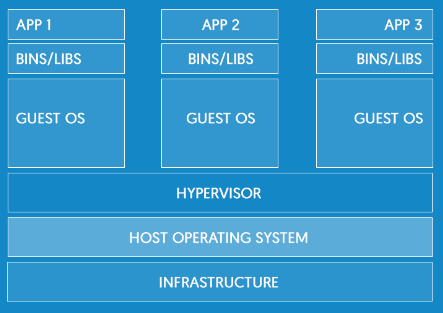
\includegraphics[width=0.4\textwidth]{VirtualBox}
	\caption{Aufbau VirtualBox}
	\label{img:AufbauVirtualBox}
\end{figure}